\section{Ilham Muhammad Ariq (1174087)}
\subsection{Instalasi Map Server}
\begin{enumerate}
	\item  Download installer Map Server pada web https://ms4w.com. Pilih yang .exe
	\hfill\break
	\begin{figure}[H]
		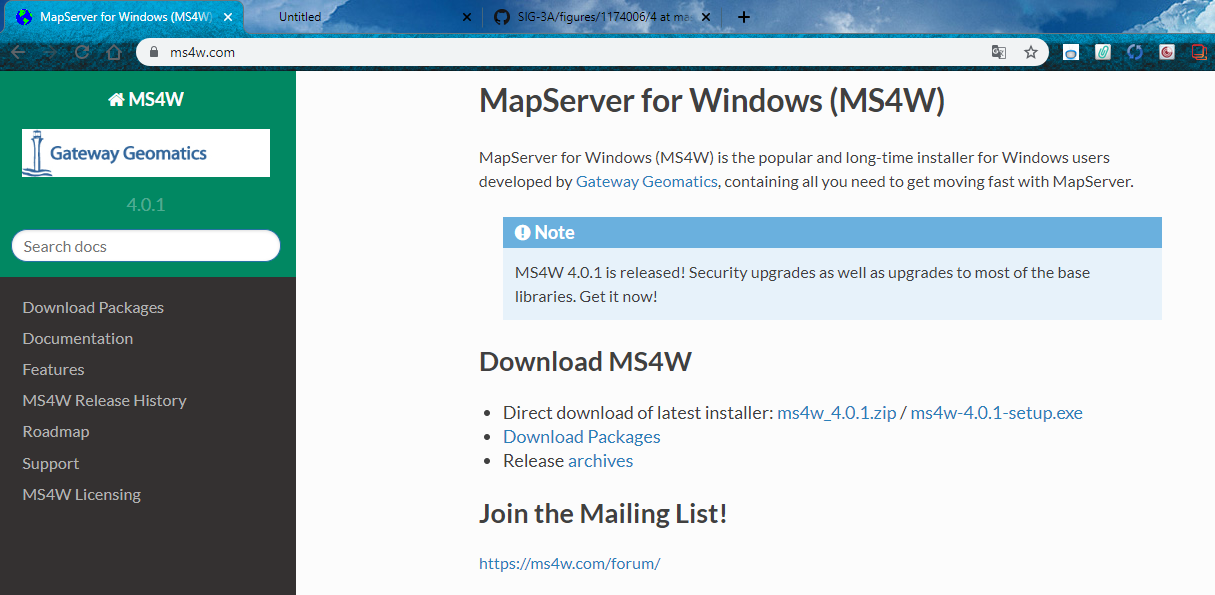
\includegraphics[width=8cm]{figures/Tugas4/1174087/1.png}
		\centering
		\caption{Download installer Map Server.}
	\end{figure}
	\item  Setelah selesai di download, Cari file download dan lakukan install aplikasi ms4w ,klik dua kali pada installer.
	\hfill\break
	\begin{figure}[H]
		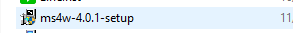
\includegraphics[width=8cm]{figures/Tugas4/1174087/2.png}
		\centering
		\caption{Klik 2x Installer}
	\end{figure}
	\item  klik "I Agree".
	\hfill\break
	\begin{figure}[H]
		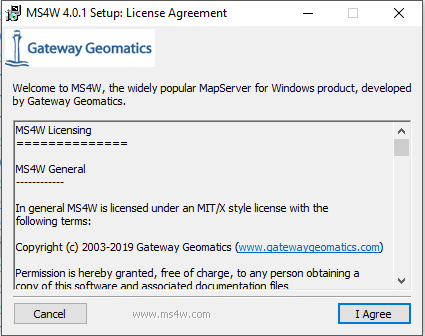
\includegraphics[width=8cm]{figures/Tugas4/1174087/3.png}
		\centering
		\caption{Klik "I Agree".}
	\end{figure}
	\item  Pilih tipe instalasi yang "Full". Kemudian klik Next.
	\hfill\break
	\begin{figure}[H]
		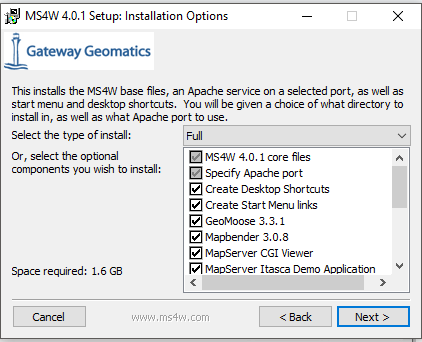
\includegraphics[width=8cm]{figures/Tugas4/1174087/4.png}
		\centering
		\caption{Tipe instalasi "Full".}
	\end{figure}
	\item  Pilih direktori instalasinya. Kemudian klik Next.
	\hfill\break
	\begin{figure}[H]
		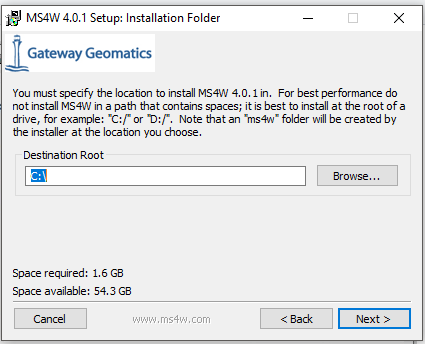
\includegraphics[width=8cm]{figures/Tugas4/1174087/5.png}
		\centering
		\caption{Pilih direktori instalasi}
	\end{figure}
	\item  Isi port Apache yang akan dipakai. Kemudian klik Next.
	\hfill\break
	\begin{figure}[H]
		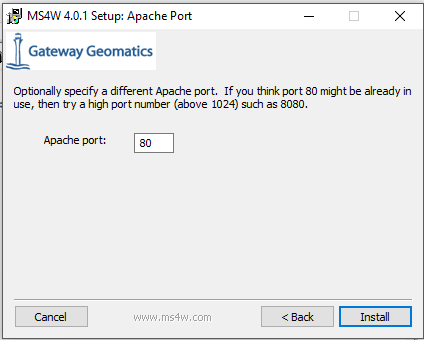
\includegraphics[width=8cm]{figures/Tugas4/1174087/6.png}
		\centering
		\caption{Isi port Apache.}
	\end{figure}
	\item  Tunggu hingga proses instalasi selesai.
	\hfill\break
	\begin{figure}[H]
		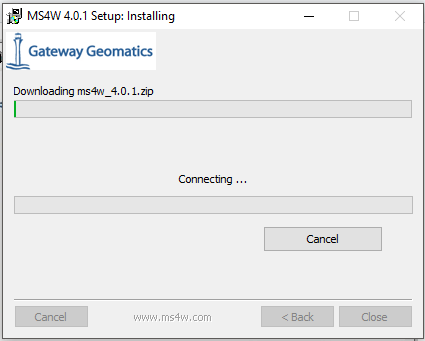
\includegraphics[width=8cm]{figures/Tugas4/1174087/7.png}
		\centering
		\caption{Proses instalasi.}
	\end{figure}
	\item  Klik Close.
	\hfill\break
	\begin{figure}[H]
		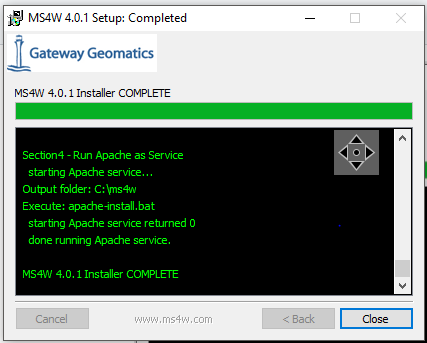
\includegraphics[width=8cm]{figures/Tugas4/1174087/8.png}
		\centering
		\caption{Akhir proses instalasi.}
	\end{figure}
\end{enumerate}
\subsection{Instalasi Map Proxy}
\begin{enumerate}
	\item  Ketik peritah berikut di CMD.
	\hfill\break
	\begin{figure}[H]
		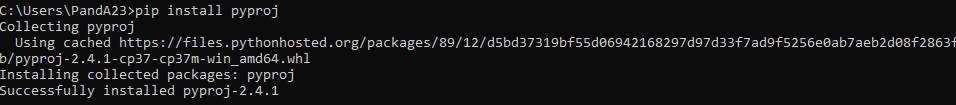
\includegraphics[width=8cm]{figures/Tugas4/1174087/11.png}
		\centering
		\caption{Install Map Proxy}
	\end{figure}
	\item  Ketik peritah berikut di CMD.
	\hfill\break
	\begin{figure}[H]
		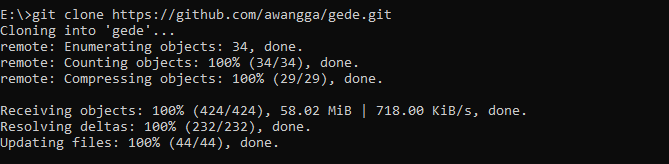
\includegraphics[width=8cm]{figures/Tugas4/1174087/12.png}
		\centering
		\caption{Install pyproj}
	\end{figure}
\end{enumerate}
\subsection{Link Youtube}
https://youtu.be/ZY5f234LOcE

\subsection{Membuka map menggunakan MapProxy}
\begin{enumerate}
  \item Download / clone git terlebih dahulu file dari https://github.com/awangga/gede
  \item Pastikan path menuju folder gede tidak ada spasi 
  \hfill\break
  \begin{figure}[H]
  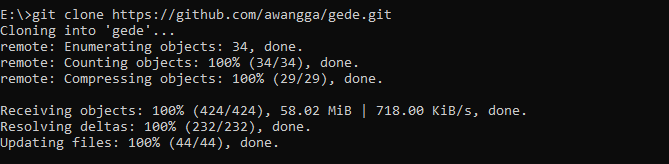
\includegraphics[width=4cm]{figures/Tugas4/1174087/12.png}
  \centering
  \caption{git clone}
  \end{figure}
  
  \item Pada folder gede buat folder bernama tmp
  \hfill\break
  \begin{figure}[H]
  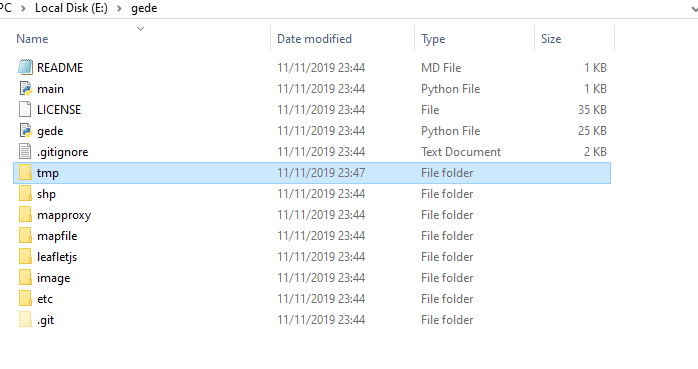
\includegraphics[width=4cm]{figures/Tugas4/1174087/13.png}
  \centering
  \caption{buat folder tmp}
  \end{figure}
 
  \item Setelah itu buka folder mapproxy lalu edit file agm.yaml menggunakan text editor contoh visual code studio
  \item Pada bagian sources lalu ada map:, masukkan pathnya sesuai dengan tempat menyimpan data clone tdi contohnya E:/gede/mapfile/mywms.map
  \hfill\break
  \begin{figure}[H]
  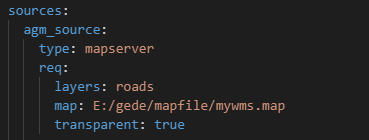
\includegraphics[width=4cm]{figures/Tugas4/1174087/14.png}
  \centering
  \caption{Edit lokasi mymap.map}
  \end{figure}


  \item Kemudian pada bagian binary masukkan lokasi instalasi ms4w yagn berada pada C:/ms4w/Apache/cgi-bin/mapserv.exe
  \item Selanjutnya pada bagian working-dir masukkan path folder temp yang telah kita buat tadi, yang saya E:/gede/tmp
  \hfill\break
  \begin{figure}[H]
  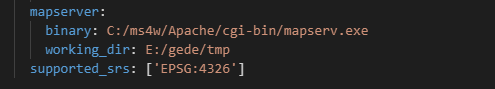
\includegraphics[width=4cm]{figures/Tugas4/1174087/15.png}
  \centering
  \caption{Edit binary dan path working-dir}
  \end{figure}

  \item Setelah itu buka aplikasi MS4W-Shell
  \item Kemudian masuk directory mapproxy pada folder clone tadi ,setelah masuk ke directorinya ketikkan "mapproxy-util serve-develop agm.yaml" pada ms4w-Shell untuk membuka aplikasi mapproxy
  \hfill\break
  \begin{figure}[H]
  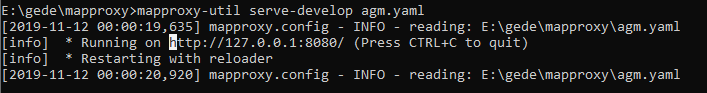
\includegraphics[width=4cm]{figures/Tugas4/1174087/16.png}
  \centering
  \caption{Buka aplikasi mapproxy}
  \end{figure}

  \item Buka browser lalu ketikkan 127.0.0.1:8080
  \hfill\break
  \begin{figure}[H]
  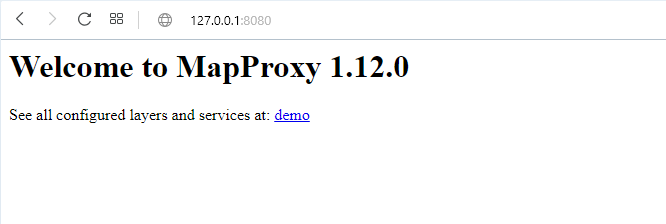
\includegraphics[width=4cm]{figures/Tugas4/1174087/17.png}
  \centering
  \caption{Buka mapproxy pada browser}
  \end{figure}

  \item lalu klik demo untuk melihat map
  \item lalu klik png pada agm, maka mapproxy akan menampilkan map
  \hfill\break
  \begin{figure}[H]
  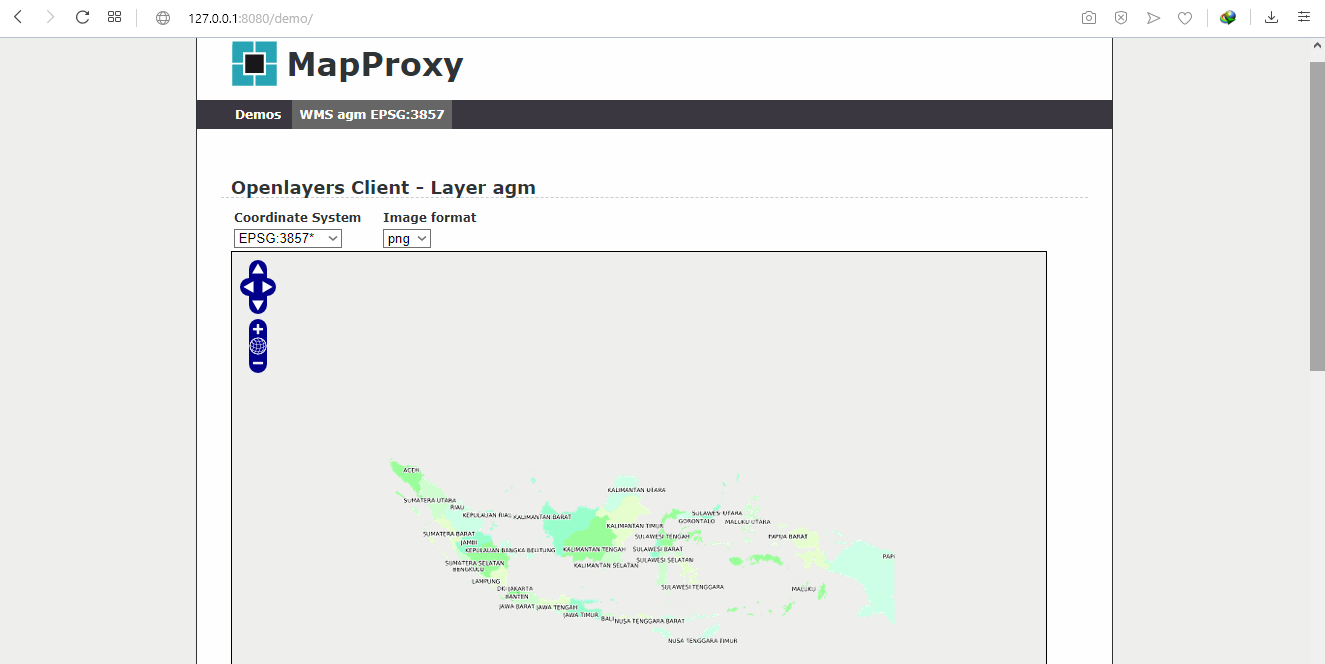
\includegraphics[width=4cm]{figures/Tugas4/1174087/18.png}
  \centering
  \caption{MapProxy menampilkan map}
  \end{figure}

\end{enumerate}

\subsection{Link Youtube}
https://youtu.be/NwbD7YG-aPI